\documentclass[UTF8]{ctexart}

\usepackage{subfiles}  

%下面的语句, 引入你的头部设置文件
\usepackage{C:/phpStorm_proj/02_myself_ID_EGO/+100_latex_all_math_sel/myPreamble} 
%必须是绝对路径,才能让各个tex在单独编译时使用到

\title{微分}


%---------------------------------


\begin{document}
	\tableofcontents % 生成目录
	\date{} % 若不写这句, 则默认也会渲染出日期, 所以我们要手动赋空值
	\maketitle  %这行代码, 让你前面的 title, author, date生效
	
	
	\section{线性主部 $dy= A \cdot \varDelta x $}
	
	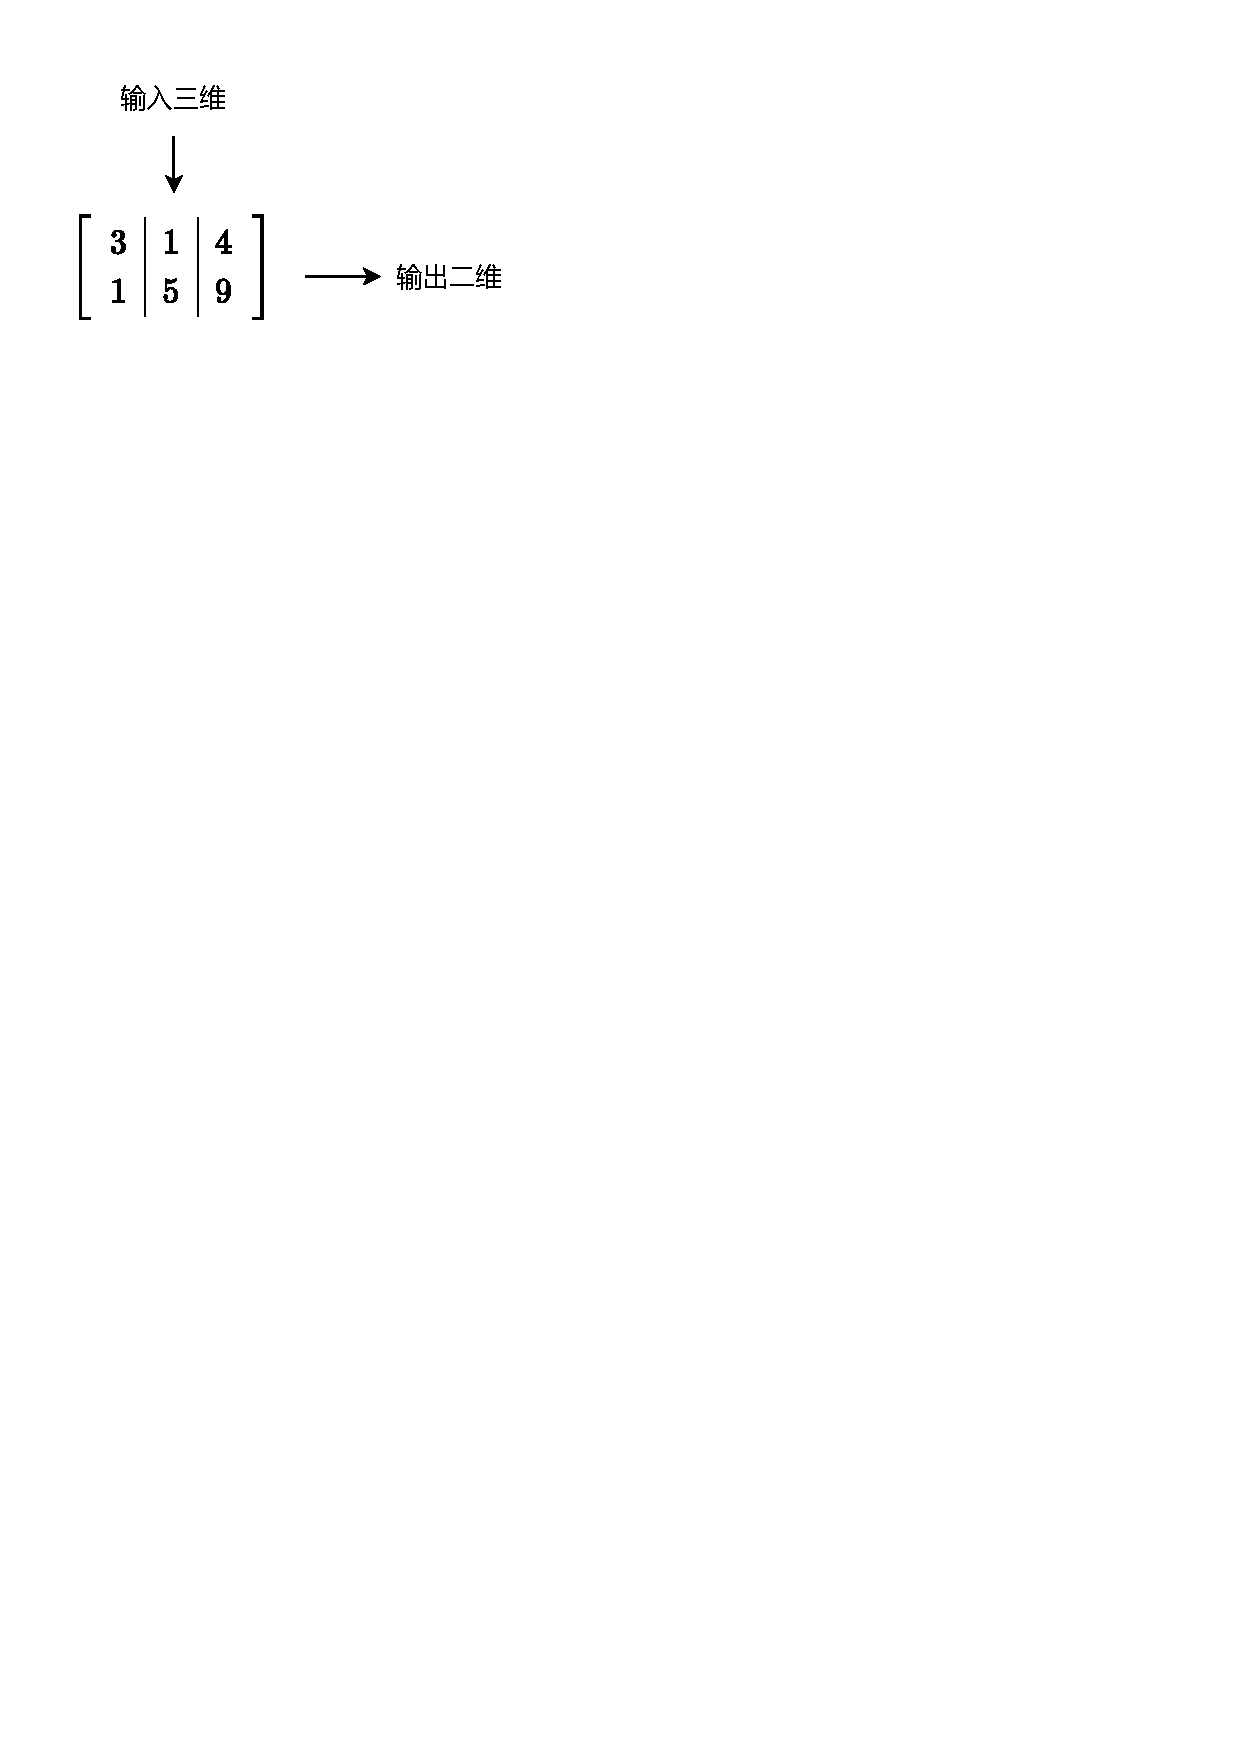
\includegraphics[width=0.6\textwidth]{/0041.pdf} 
	
	
	黄色的矩形面积, 往外扩充增加的面积 
	$ 	
	\varDelta S =\underset{\text{整个大矩形面积}}{\underbrace{\left( x_0+\varDelta x \right) ^2}}-\underset{\text{原先的黄色矩形面积}}{\underbrace{\left( x_0 \right) ^2}}
	$ \\
	
	当Δx的距离→0 时, 红色小矩形面积 $(\Delta x)^2$ 的值可以忽略不计.
	
	即:
	
	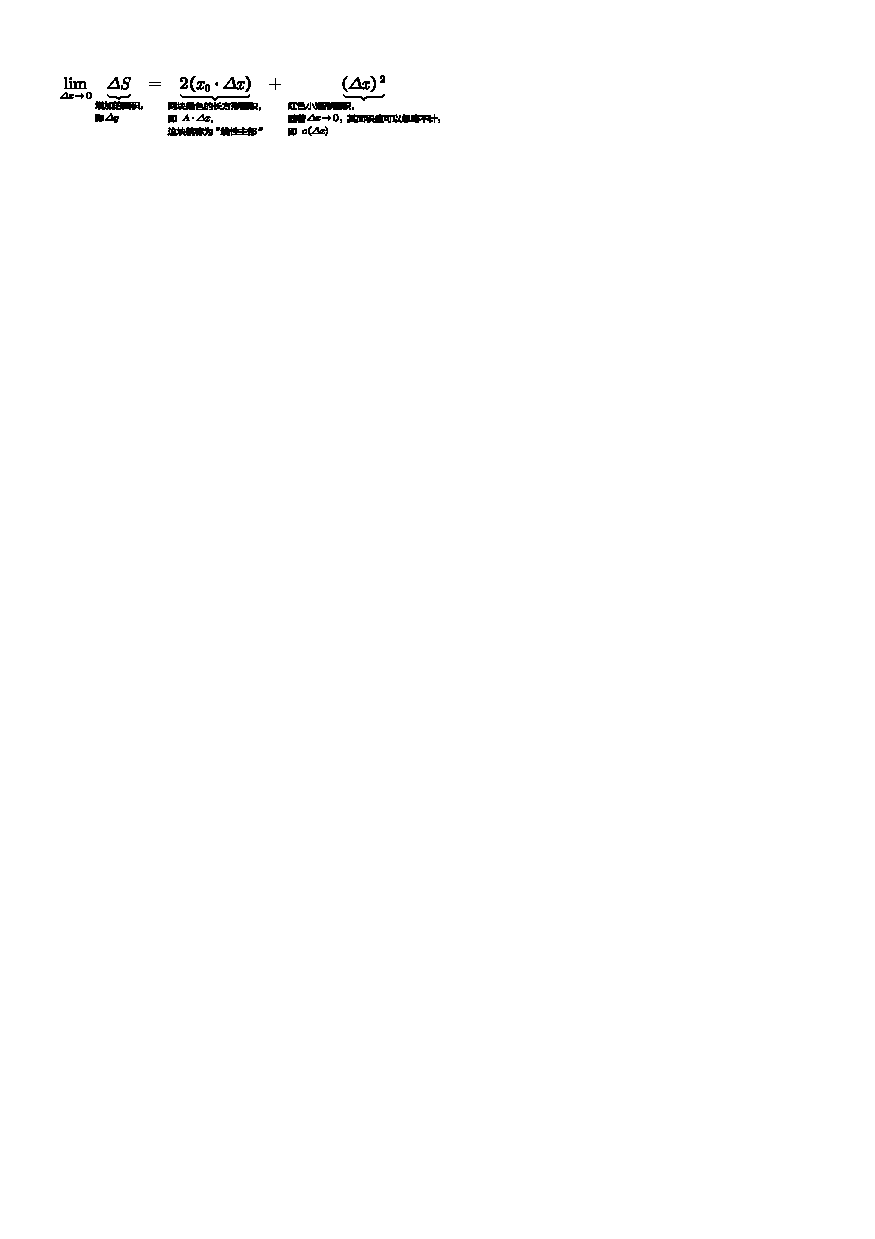
\includegraphics[width=0.7\textwidth]{/0042.pdf}
	
	\textbf{所以原始黄色矩形增加的面积, 主要取决于 AΔx (即两块绿色长方形面积之和) 这块``线性主部"的变化值.}
	
	所以:
	
	→ 函数变化的``精确值"是: $\varDelta y=\underset{\text{线性主部}}{\underbrace{A\varDelta x}}+ o\left( \varDelta x \right)  $ ← 其中 o(Δx) 是比 Δx 高阶的无穷小.
	
	→ 函数变化的``近似值"是: $dy=\underset{\text{线性主部}}{\underbrace{A\varDelta x}} $ \\
	
	$A \Delta x$ : 这里面, 变化的只是Δx, 而A可以看成是一个``常数".
	
	$o\left( \varDelta x \right) $ : 它是比 Δx 高阶的无穷小. 即它比 Δx 趋近于0的速度更快. 如下图所示: \\
	
	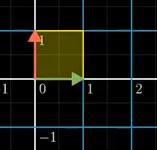
\includegraphics[width=0.3\textwidth]{/0043.png}
	
	
	
	
	
	~\\
	\hrule
	~\\
	
	
	
	\section{当$\varDelta x \rightarrow 0 $ 时, 我们可以用 切线的高度 dy (即``微分"), 来代替曲线的高度 Δy.}
	
	
	我们可能想去求曲线的长度、曲线下的面积. 解决思路是这样的 : 比如, 求曲线长度,我们就将曲线分为一小段一小段,每一小段, 都用切线来近似该段曲线:\\
	
	
\includegraphics[width=0.35\textwidth]{/0045.png}
	
	分段的越细,直到划分为无穷多份,这些切线的长度加起来, 就是曲线的长度. \\
	
	\textbf{对于每一段的``曲线"本身, 和该段区间中的``切线", 可以看到, 在Δx尽可能小的距离内 (即在 $\left( x_0-\varDelta x,\ x_0+\varDelta x \right) $ 的区间内), 曲线 f(x)的高度, 和 其切线(直线)g(x)的高度, 相差很小.} 所以, 当 $\varDelta x \rightarrow 0 $ 时, 我们就可以用 dy, 来代替 Δy. \\
	
	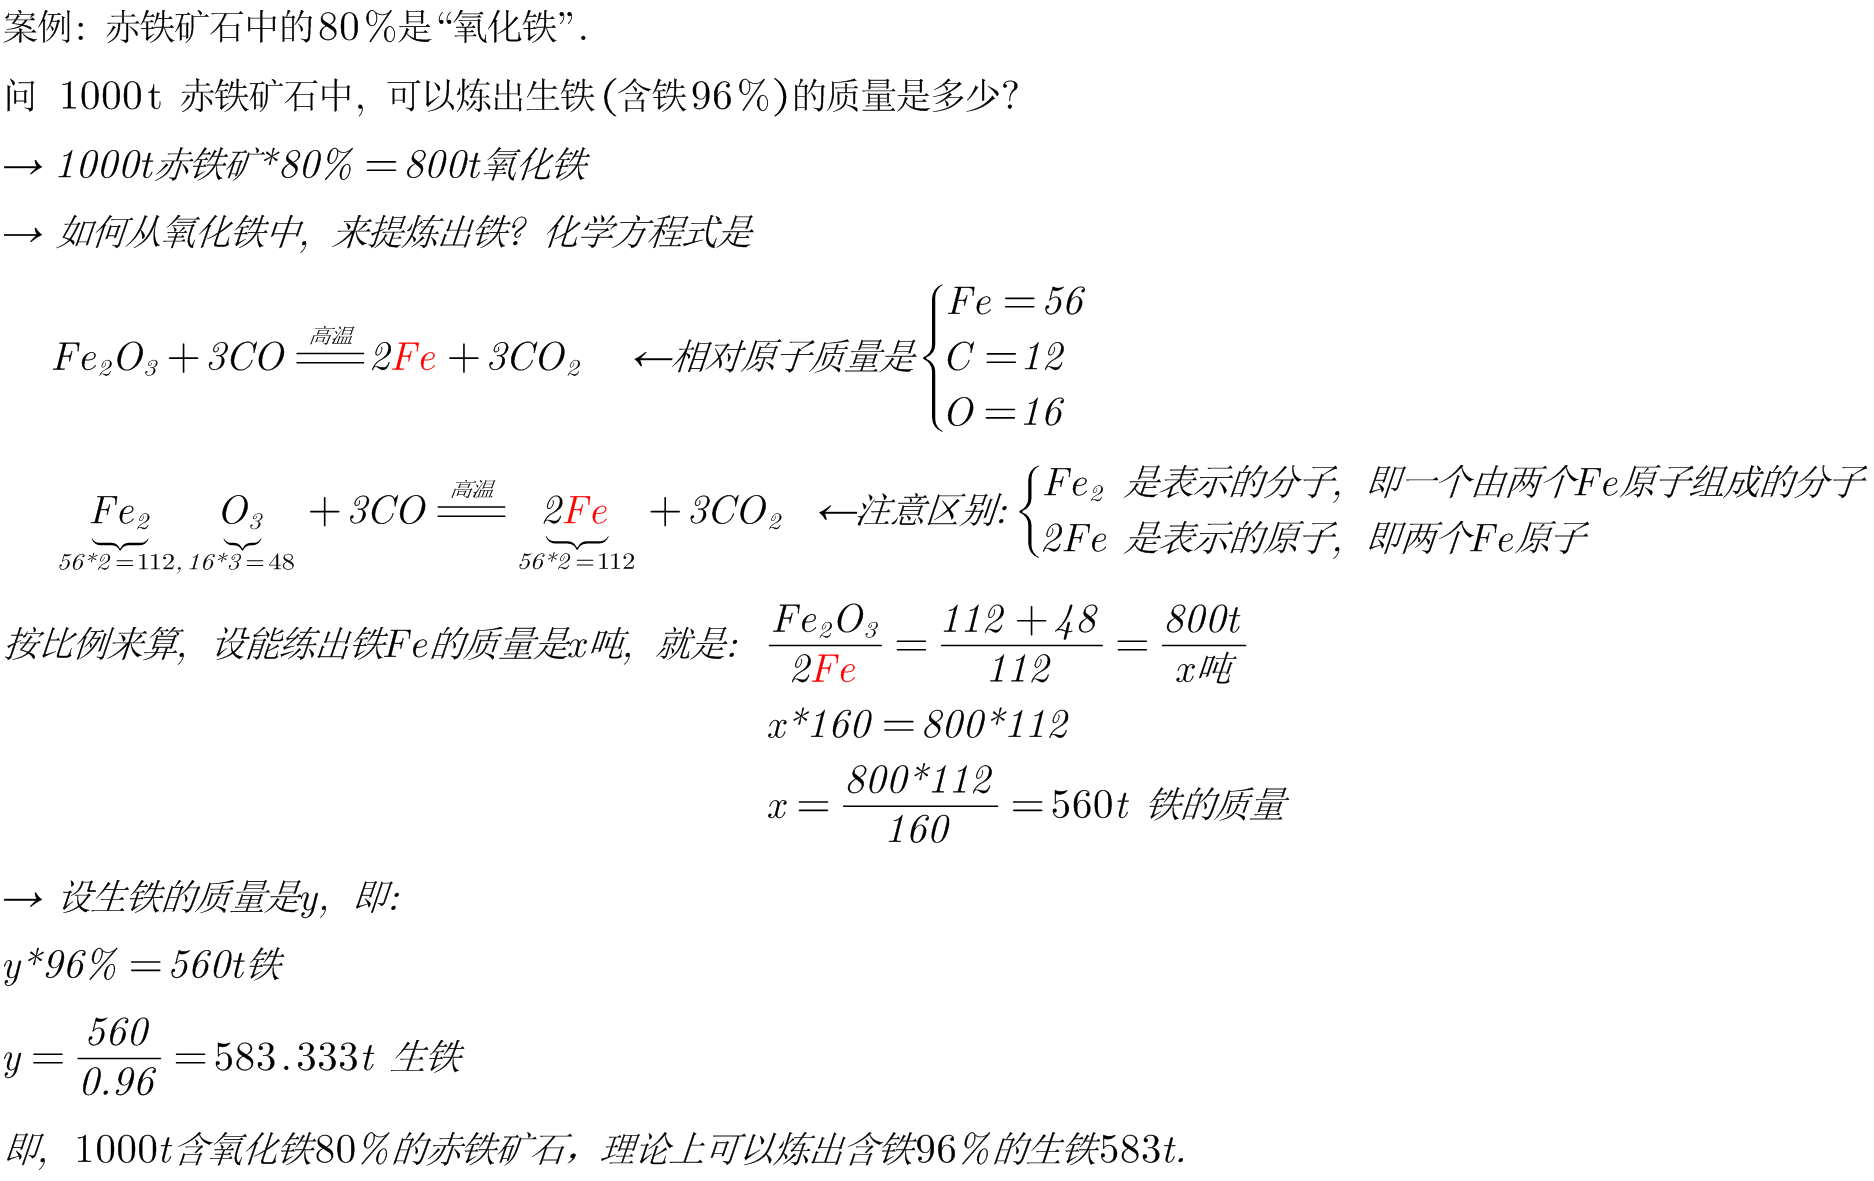
\includegraphics[width=0.35\textwidth]{/0046.png} \\
	
	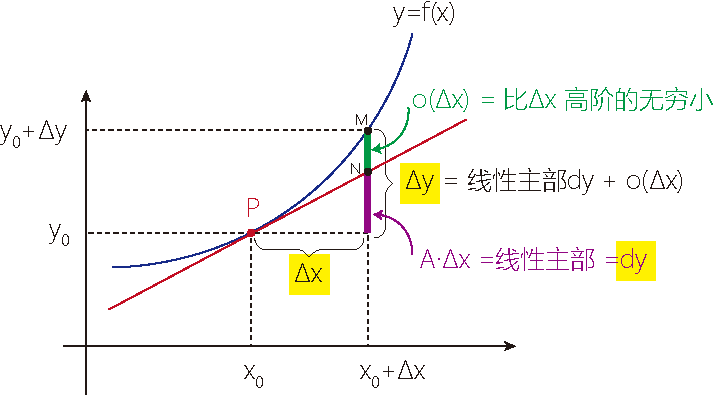
\includegraphics[width=0.6\textwidth]{/0044.pdf} \\
	
	
	所以: 如果函数的增量 $\varDelta y=f\left( x+\varDelta x \right) -f\left( x \right) $ 可表示为 Δy = AΔx + o(Δx) (其中A是不随Δx 改变的常量, 但A可以随 x 改变), 而o(Δx)是比Δx高阶的无穷小 (注: o 是希腊字母 omicron). 我们就能称: y=f(x) 在 $x_0$点处``可微".  \\
	
	把 dy, 称作y=f(x) 在 $x_0$点处的``微分". $dy=A\varDelta x$. 换言之, \textbf{函数的``微分", 就是函数增量(即 Δy)的主要部分(即``线性主部"部分, 即 dy部分).}  记作: $dy\mid_{x=x_0}^{}=A\cdot \varDelta x$ \\

	即:
	
	- ``函数f 的自变量x" 的微分, 就是dx. 其值是: dx = Δx.  ← 这两个是精确相等的, 就是一回事.
	
	- ``函数f 的y值"的微分, 就是 dy. 其值是: dy = Δy的``线性主部"部分 = AΔx = 函数 f(x) 在 $x_0$ 点处的``微分".  ← dy 只是 Δy 的近似. \\
	
	所以, ``微分"dy 的本质, 就是用一个``线性函数"(即切线) 作为``原函数"变化的逼近。 即 用 dy(近似值) 来代替 Δy(精确值).  \\
	
	
	
	进一步:

	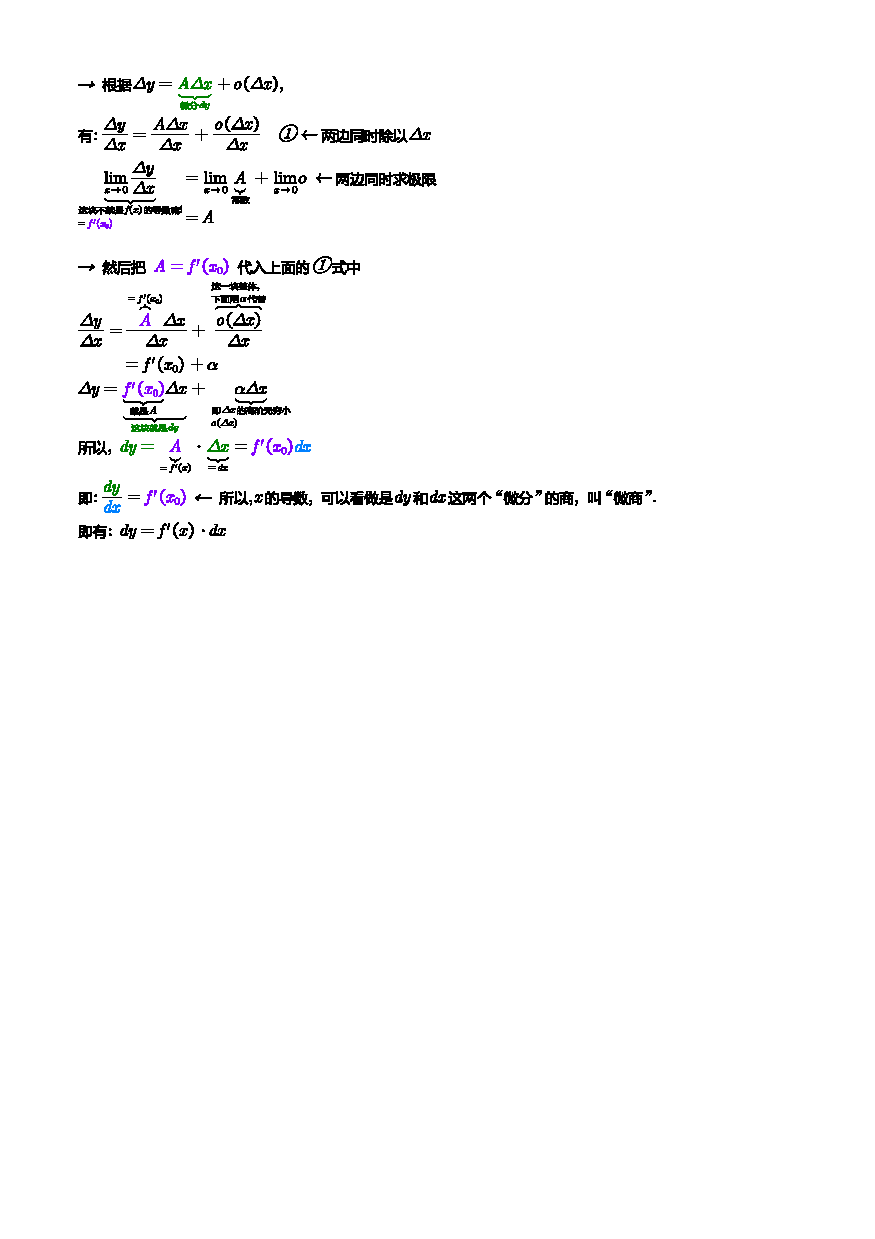
\includegraphics[width=0.9\textwidth]{/0047.pdf}
	
	所以, 我们就得到了 求``微分 dy 或 df(x)"这个值的公式: $ \boxed{ dy= f'(x) \cdot dx}$ \\
	
	微分 dy 的几何意义:  $dy=f'\left( x \right) \varDelta x$ 就是函数 f(x) 在x点处的 ``切线纵坐标"的改变量. 随着 Δx 的距离趋向于(缩小为)0, dy=Δy. \\
	
	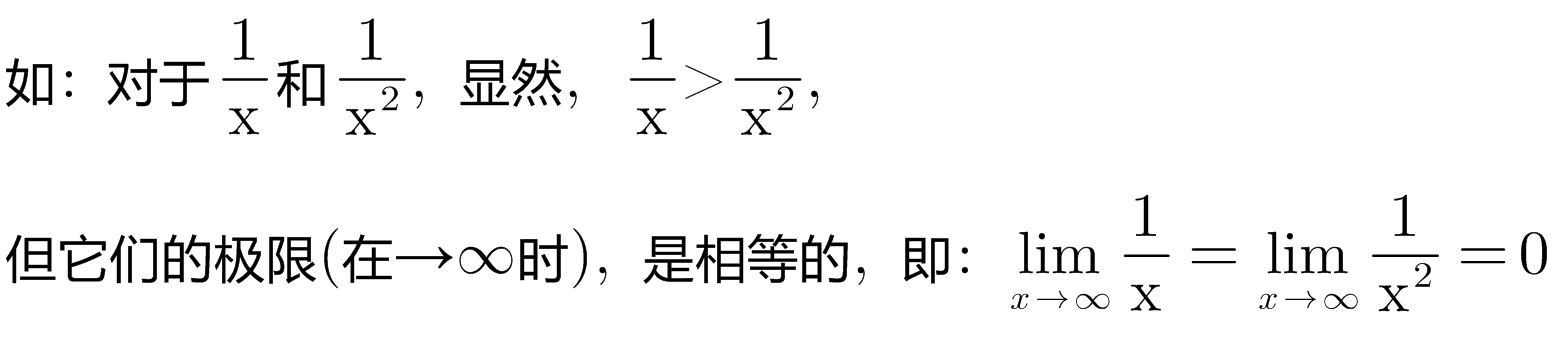
\includegraphics[width=0.4\textwidth]{/0048.png}	\\
	
	
	\begin{myEnvSample}
		\begin{align*}
	&y=x^2,\ \text{求}x=1,x=3\text{这两处的微分}.\\
&\text{根据微分公式:\ }dy=f'\left( x \right) dx,\text{我们先要知道}f'\left( x \right) \text{和}dx\text{这两个数值}\\
&\rightarrow \ y=x^2\text{的导数, 即}y'=2x\\
&\rightarrow \ dx=\varDelta x\\
&\text{所以,微分}dy=\underset{=2x}{\underbrace{f'\left( x \right) }}\underset{=\varDelta x}{\underbrace{dx}}\\
&\text{当}x=1\text{时,} \ dy=2\cdot \left( 1 \right) \cdot \varDelta x=2\varDelta x\\
&\text{当}x=3\text{时,} \ dy=2\cdot \left( 3 \right) \cdot \varDelta x=6\varDelta x
		\end{align*}
	\end{myEnvSample}
	
	
	\begin{myEnvSample}
		\begin{align*}
	&y=x^3,\ \text{已知}\varDelta x=0.02,\ \text{求}x=2\text{处的微分}dy\\
&\text{根据微分公式:\ }dy=f'\left( x \right) dx\\
&\text{本例就是\ }dy=\left( x^3 \right) '\underset{=\varDelta x}{\underbrace{dx}}=3x^2\underset{=0.02}{\underbrace{\varDelta x}}\ \gets \text{把}x=2\text{代入进去}\\
&dy=3\left( 2 \right) ^2\cdot 0.02=0.24
		\end{align*}
	
	注意: 因为这里Δx有个具体的值0.02, 所以Δx没有趋近于0. 即这里求得的dy, 就是``切线"的y值增量, 而非``函数曲线本身"的y值增量.
	\end{myEnvSample}
	
	
	所以:
	
	- 函数曲线 y的变化量的 ``精确值"是 $\Delta y = f(x_0 + \Delta x) - f(x_0)$
	
	- y的变化量的 ``近似值"是 $dy=f'\left( x_0 \right) \cdot \underset{=\varDelta x}{\underbrace{dx}}$
	
	即, dy ≈ Δy, 所以, 曲线变化后的y高, 即:
	
	 $f\left( x_0+\varDelta x \right) \approx \underset{\text{曲线在}x_0\text{处的}y\text{高}}{\underbrace{f\left( x_0 \right) }}+\underset{\text{切线的}y\text{值增加量}}{\underbrace{\text{微分}dy}}=f\left( x_0 \right) +\underset{\text{即微分}dy}{\underbrace{f'\left( x_0 \right) \cdot \varDelta x}}$ \\
	\\
	
	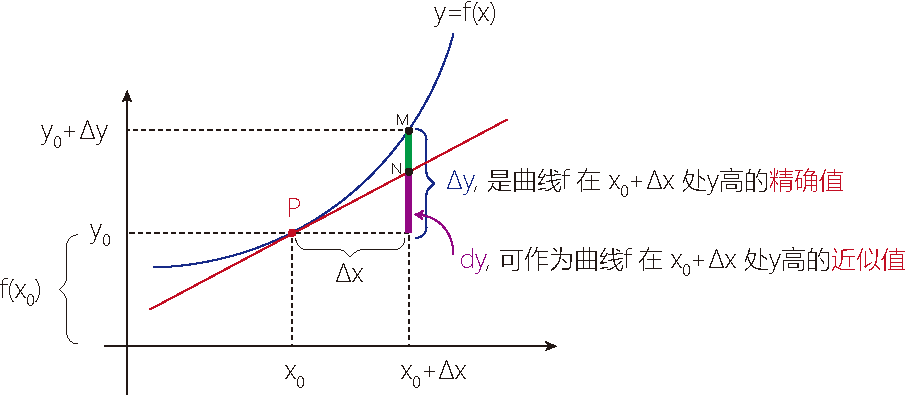
\includegraphics[width=0.8\textwidth]{/0049.pdf}
	
	
	\begin{myEnvSample}
		有一个半径为 1cm 的球, 在表面镀铜 0.01cm 厚, 问: 所镀的铜的体积是多少?
		
		球的体积公式是 $V=\frac{4}{3}\pi r^3$, 我们要求的就是 ΔV. 那我们就用 dy 来近似 Δy :			
		
		\begin{align*}
	&\text{根据微分公式\ }dy=\underset{\text{本例函数的}y,\ \text{即体积}V'}{\underbrace{f'\left( x_0 \right) }}\cdot \underset{\text{本例函数的自变量}x,\text{即球体的半径}r}{\underbrace{dx}}\\
&dy=\left( \frac{4}{3}\pi \underset{\text{本例的}r=1cm}{\underbrace{r^3}} \right) '\cdot \underset{=\text{增加了}0.01cm\text{半径}}{\underbrace{\varDelta x}}\\
&=\frac{4}{3}\pi \cdot 3\left( 1 \right) ^2\cdot 0.01=0.125664\ cm^3\\
		\end{align*}
	\end{myEnvSample} 



\begin{myEnvSample}
	角度中的``度分秒制"是: 1度=60分, 1分=60秒 (度 $^\circ$ , 分', 秒'')
	
	求 $\sin \left( 30^\circ 30' \right) $
	\begin{align*}
	&\begin{matrix}
	\sin \left( 30^{\circ}30' \right) =\sin \left( \underset{\text{可看成是}x_0}{\underbrace{\frac{\pi}{6}}}+\underset{\text{可看成是}\varDelta x}{\underbrace{\frac{\pi}{360}}} \right)\\
\end{matrix}\\
&\text{根据公式:\ 曲线新的}y\text{高}\approx \underset{\text{曲线在原先点上的高度}}{\underbrace{f\left( x_0 \right) }}+\underset{\text{切线的}y\text{值增量}}{\underbrace{dy}}\\
&=\sin \left( \frac{\pi}{6} \right) +\underset{\text{微分}dy}{\underbrace{\left[ \underset{\text{即}\left( \sin \frac{\pi}{6} \right) '}{\underbrace{f'\left( x_0 \right) }}\cdot \underset{=\varDelta x=30'=\frac{\pi}{360}}{\underbrace{dx}} \right] }}=\sin \left( \frac{\pi}{6} \right) +\left( \sin \frac{\pi}{6} \right) '\cdot \frac{\pi}{360}=0.5076
	\end{align*}
\end{myEnvSample}
	

可以看出, 微分这种方法, 其实就是我们把一个数(比如我们算一个函数值), 分成两块来分别对待, 比如拆分成``整数部分"和``小数部分". 整数部分(占大头), 就算出它的精确值; 小数部分(占小头, 所以稍微有点误差, 也没关系), 就用"近似值"来代表它.  这样组合后, 算出的结果, 和精确值就相差不大.



~\\
\hrule
~\\	


\section{常用近似值}

\subsubsection{$\lim_{x\rightarrow 0}\left( 1+x \right) ^n\approx 1+nx$}

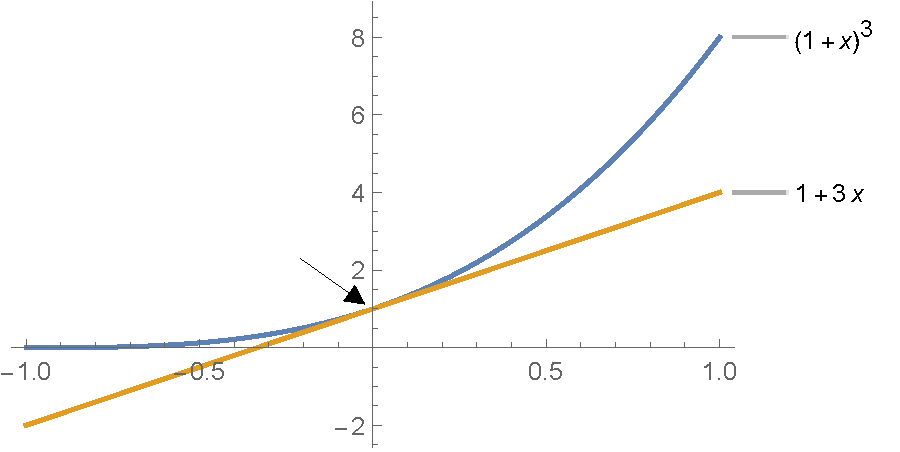
\includegraphics[width=0.5\textwidth]{/0050.pdf}



\subsubsection{$\lim_{x\rightarrow 0}\sin x\approx x$}


\subsubsection{$\lim_{x\rightarrow 0}\tan x\approx x$}

\subsubsection{$\lim_{x\rightarrow 0}e^x\approx 1+x$}

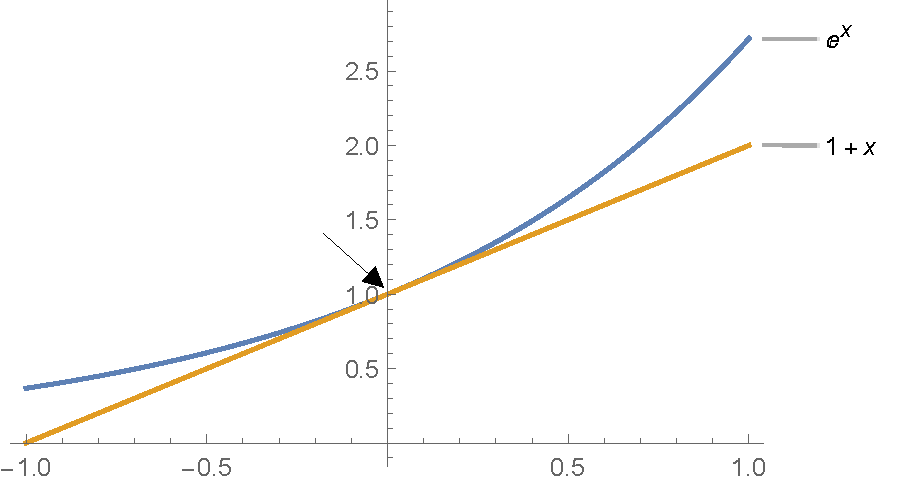
\includegraphics[width=0.5\textwidth]{/0051.pdf}



\subsubsection{$\lim_{x\rightarrow 0}\ln \left( 1+x \right) \approx x$}

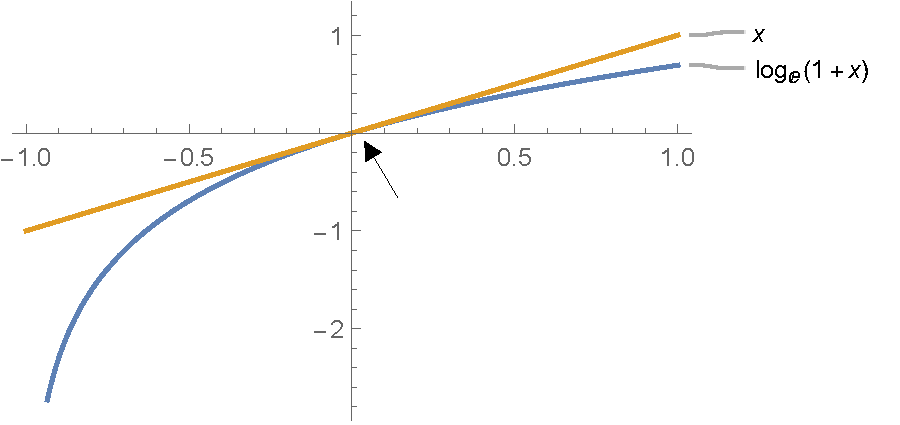
\includegraphics[width=0.5\textwidth]{/0052.pdf}

上面这些快捷计算公式, 其意义就是: 能帮助我们用(等号右边的) x 的多项式, 来近似计算(等号左边的)复杂的函数.


~\\
\hrule
~\\	


	
	
	
\section{基本微分公式与法则 : $dy = f'(x) dx$}
	
基本微分公式的核心, 依然是基于这个微分公式: $dy = f'(x) dx$

\textbf{所以, 我们把各种函数, 代入 dy中的 y部分 就行了.} 即:

例如, 对于 $x^u$ 这个函数, 它的微分就是: 我们把该函数代入 dy 中的y, 就是: $d\underset{x^u}{\underbrace{y}}=\underset{\left( x^u \right) '}{\underbrace{f'\left( x \right) }}dx$, 就得到 $d\left( x^u \right) =ux^{u-1}dx$ \\
	
同样: sin x 的微分就是: $d\underset{\sin x}{\underbrace{y}}=\underset{\left( \sin x \right) '}{\underbrace{f'\left( x \right) }}dx$, 就得到 $d\left( \sin x \right) =\cos x\ dx$ \\

\begin{myEnvSample}
	\begin{align*}
	&\text{求\ }y=\sin \left( 2x+1 \right) \ \text{的微分}dy\\
&\text{根据微分公式\ }dy=f'\left( x \right) dx\\
&\text{本例}dy=\underset{\text{复合函数求导,\ 用剥洋葱法}}{\underbrace{\left[ \sin \left( 2x+1 \right) \right] '}}dx\\
&=\left[ \sin\text{'}\left( 2x+1 \right) \cdot \left( 2x+1 \right) ' \right] dx\\
&=\left[ \cos \left( 2x+1 \right) \cdot 2 \right] dx
	\end{align*}
\end{myEnvSample}




\subsection{微分法则}
	
	\subsubsection{$d\left( \text{常数}C\cdot u \right) =\text{常数}C\cdot du$}
	
		
	\subsubsection{$d\left( \text{前}\pm \text{后} \right) =\left( \text{前}\pm \text{后} \right) 'dx=d\text{前}\pm d\text{后}	$}
	
	\subsubsection{$d\left( \text{前}\cdot \text{后} \right) =\left( \text{前}\cdot \text{后} \right) 'dx=d\text{前}\cdot \text{后}+\text{前}\cdot d\text{后}	$}
	
	\subsubsection{$d\left( \frac{\text{子}}{\text{母}} \right) =\left( \frac{\text{子}}{\text{母}} \right) 'dx=\dfrac{\text{子'}\cdot \text{母}-\text{子}\cdot \text{母'}}{\text{母}^2}dx=\dfrac{\left( d\text{子}\cdot \text{母} \right) -\left( \text{子}\cdot d\text{母} \right)}{\text{母}^2}	$}


	
	
~\\
\hrule
~\\	
	
	
	
\section{微分学中, 有三个``中值定理" : Rolle, Lagrange, Cauchy}	
	
	
	\subsection{罗尔 Rolle 中值定理}		
	
	Rolle 中值定理就是说:  如果 R 上的函数 f(x) , 满足以下3个条件:
	
	1. 在闭区间 [a,b] 上连续 (连续, 就是必须一笔画出) 
	
	2. 在开区间 (a,b) 内可导 (可导, 就是曲线必须光滑, 不能有锐角) 
	
	3. a,b点处的 y 值相等, 即 f(a)=f(b) \\
	
	则有: 在 x轴上至少会有这样一个点 ξ 存在 : 它 ∈(a,b), 并且它的y值的导数=0, 即 f'(ξ)=0 ← 也就是说, 它切线的斜率=0, 是水平的切线. \\
	
	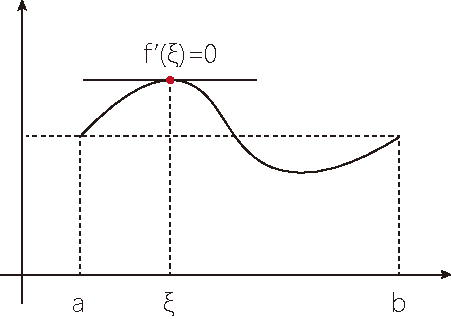
\includegraphics[width=0.4\textwidth]{/0053.pdf}
	
	简言之: 罗尔中值定理 Rolle's theorem 就是说 :  x轴上, 如果 a,b 两点的高度相同(即y值相同), 则 a,b范围内, 必能找到至少一个点c, 它(c)的切线的斜率=0, 即是水平的切线.
	
	
	
	\subsection{拉格朗日 Lagrange 中值定理}	
	
	拉格朗日中值定理, 只不过是``罗尔Rolle中值定理"的一种特殊形式而已.
	
	该定理是说, 如果函数f(x)满足: 
	
	1.在闭区间[a,b]上连续 
	
	2.在开区间(a,b)上可导  \\
	
	则就有: 在x轴上的开区间(a,b)内, 一定会存在至少一个点(如点c), 它的切线的斜率 $f'(c)$, 会和 ab直线的斜率完全相等. 即也就是有:  $\underset{\text{点}c\text{的切线斜率}}{\underbrace{f'\left( c \right) }}=\underset{ab\text{直线的斜率}}{\underbrace{\frac{f\left( b \right) -f\left( a \right)}{b-a}}}$
	
	它反映了``可导函数" 在闭区间上的``整体的平均变化率"与区间内``某点的局部变化率"的关系。 \\
	
	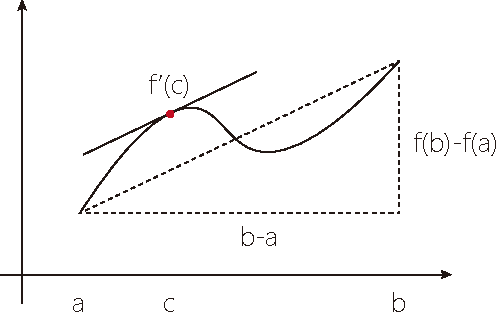
\includegraphics[width=0.4\textwidth]{/0054.pdf}	
	
	
	简言之: 拉格朗日中值定理 Lagrange mean value theorem 就是说 : x轴上 a,b范围内的曲线, 一定能找到至少一个点c, 它(c)的切线的斜率, 就等于 ab直线的斜率.
	
	
	
	\subsection{柯西 Cauchy 中值定理}	
	
	柯西中值定理, 是把``拉格朗日中值定理"中的曲线方程, 改成了``参数方程"的形式来做了. 换言之, 柯西中值定理, 可看作是``拉格朗日中值定理"的推广. 
	

	
	
\end{document}


